\documentclass[]{article}
\usepackage{graphicx}
\usepackage{float}
\usepackage[left=1.4cm, right=1.4cm, top=1.9cm, bottom=1.9cm]{geometry}
\usepackage{colortbl}
\usepackage{booktabs}


\newcolumntype{C}{>{$}c<{$}}
\AtBeginDocument{
	\heavyrulewidth=.08em
	\lightrulewidth=.05em
	\cmidrulewidth=.03em
	\belowrulesep=.65ex
	\belowbottomsep=0pt
	\aboverulesep=.4ex
	\abovetopsep=0pt
	\cmidrulesep=\doublerulesep
	\cmidrulekern=.5em
	\defaultaddspace=.5em
}

%opening
\title{STK-IN4300 Project 2}
\author{Steinn Hauser Magnusson}

\begin{document}

\maketitle

\section*{Exercise 1}
\subsection*{1.}
Section one is mostly about implementing some code. This has been done in the first function of the 'Exercise1' class. The scaling is done typically, where the mean and standard deviations of the non-categorical variables should be zero and one, respectively. The main concern of the scaling is whether or not to one-hot encode the categorical variables. All the categorical variables presented in the data are binary, such that the one-hot encoding is not computationally efficient. If these columns were to be one hot encoded, then we would be left with two columns which are highly correlated, as one column could be derived from the other. One-hot encoding of the binary categorical data is therefore not done.

\subsection*{2.}
Following are figures illustrating the Covariance and Correlation matrices of the data. A specific figure is also generated of the 'FFVC' column. Figure \ref{fig:covE1} illustrates the covariance matrix of the data:
\begin{figure}[H]
	\centering
	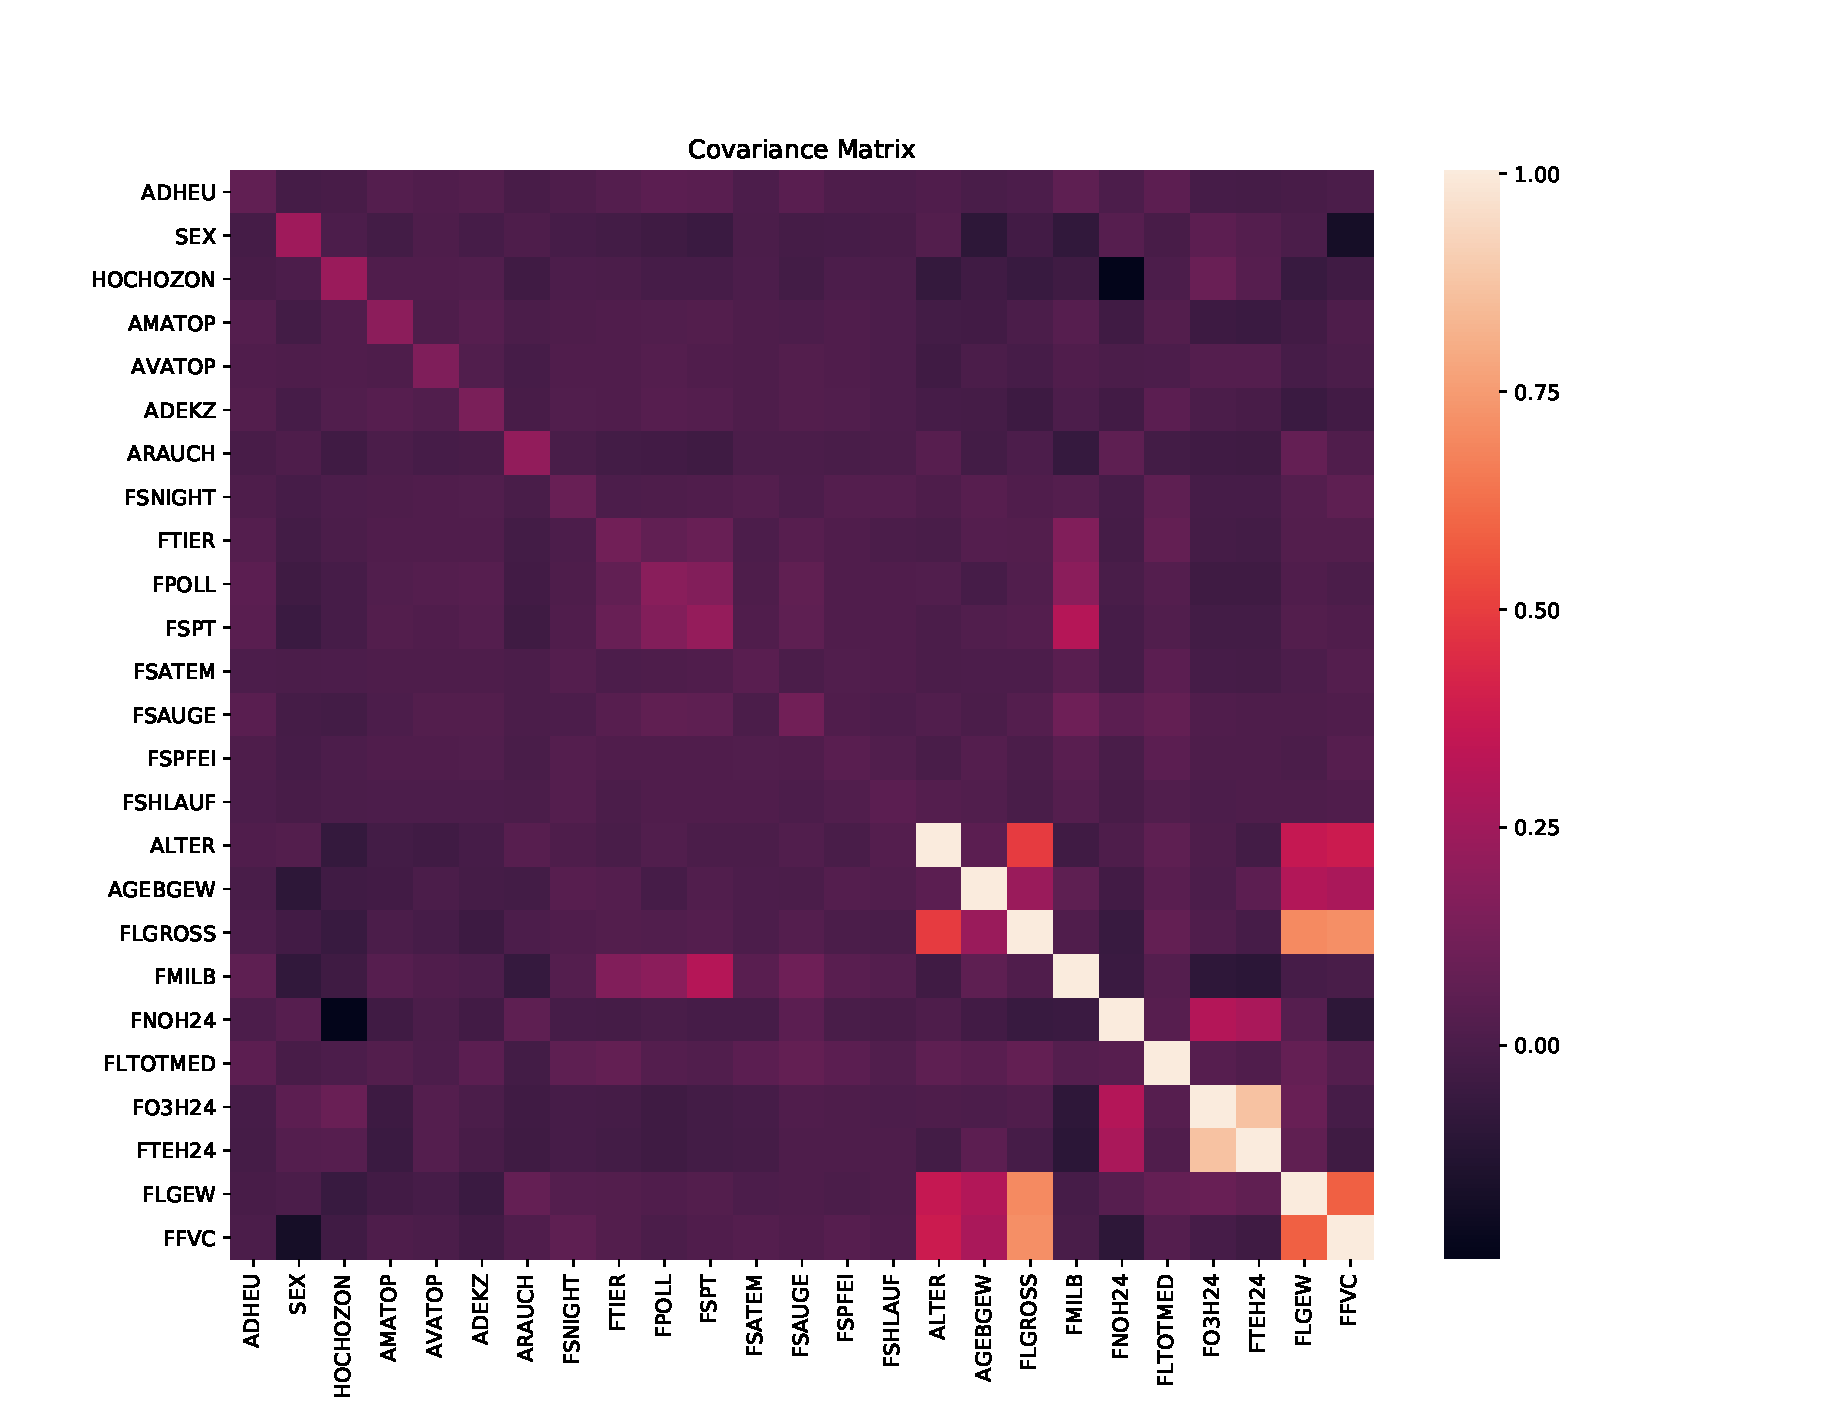
\includegraphics[width=0.8\textwidth]{figures/covheatmap.pdf}
	\caption{The covariance matrix of the data}
	\label{fig:covE1}
\end{figure}
Figure \ref{fig:cov_FFVC_E1} illustrates the covariance vector of the FFVC feature:
\begin{figure}[H]
	\centering
	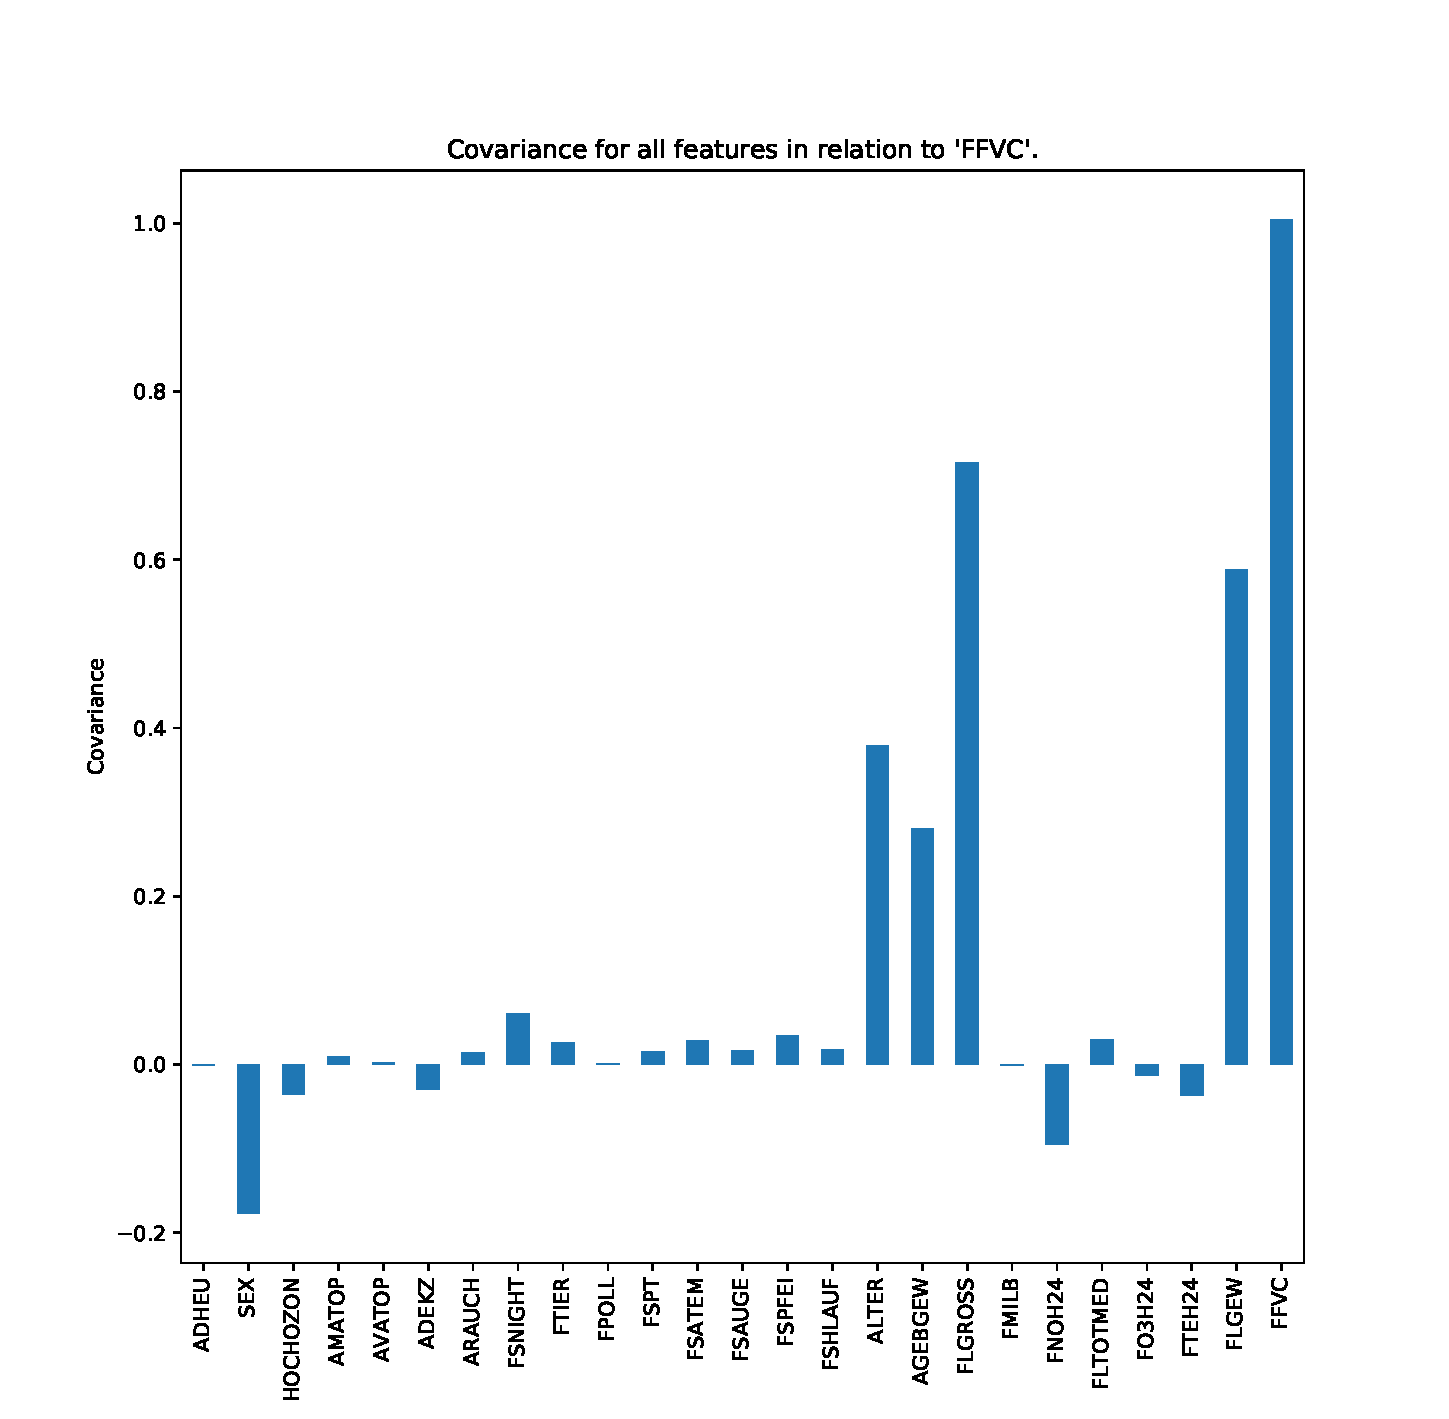
\includegraphics[width=0.8\textwidth]{figures/cov_FFVC_specific.pdf}
	\caption{The specific covariance of the FFVC features.}
	\label{fig:cov_FFVC_E1}
\end{figure}
%Figure \ref{fig:corrE1} illustrates the correlation matrix of the data:
%\begin{figure}[H]
%	\centering
%	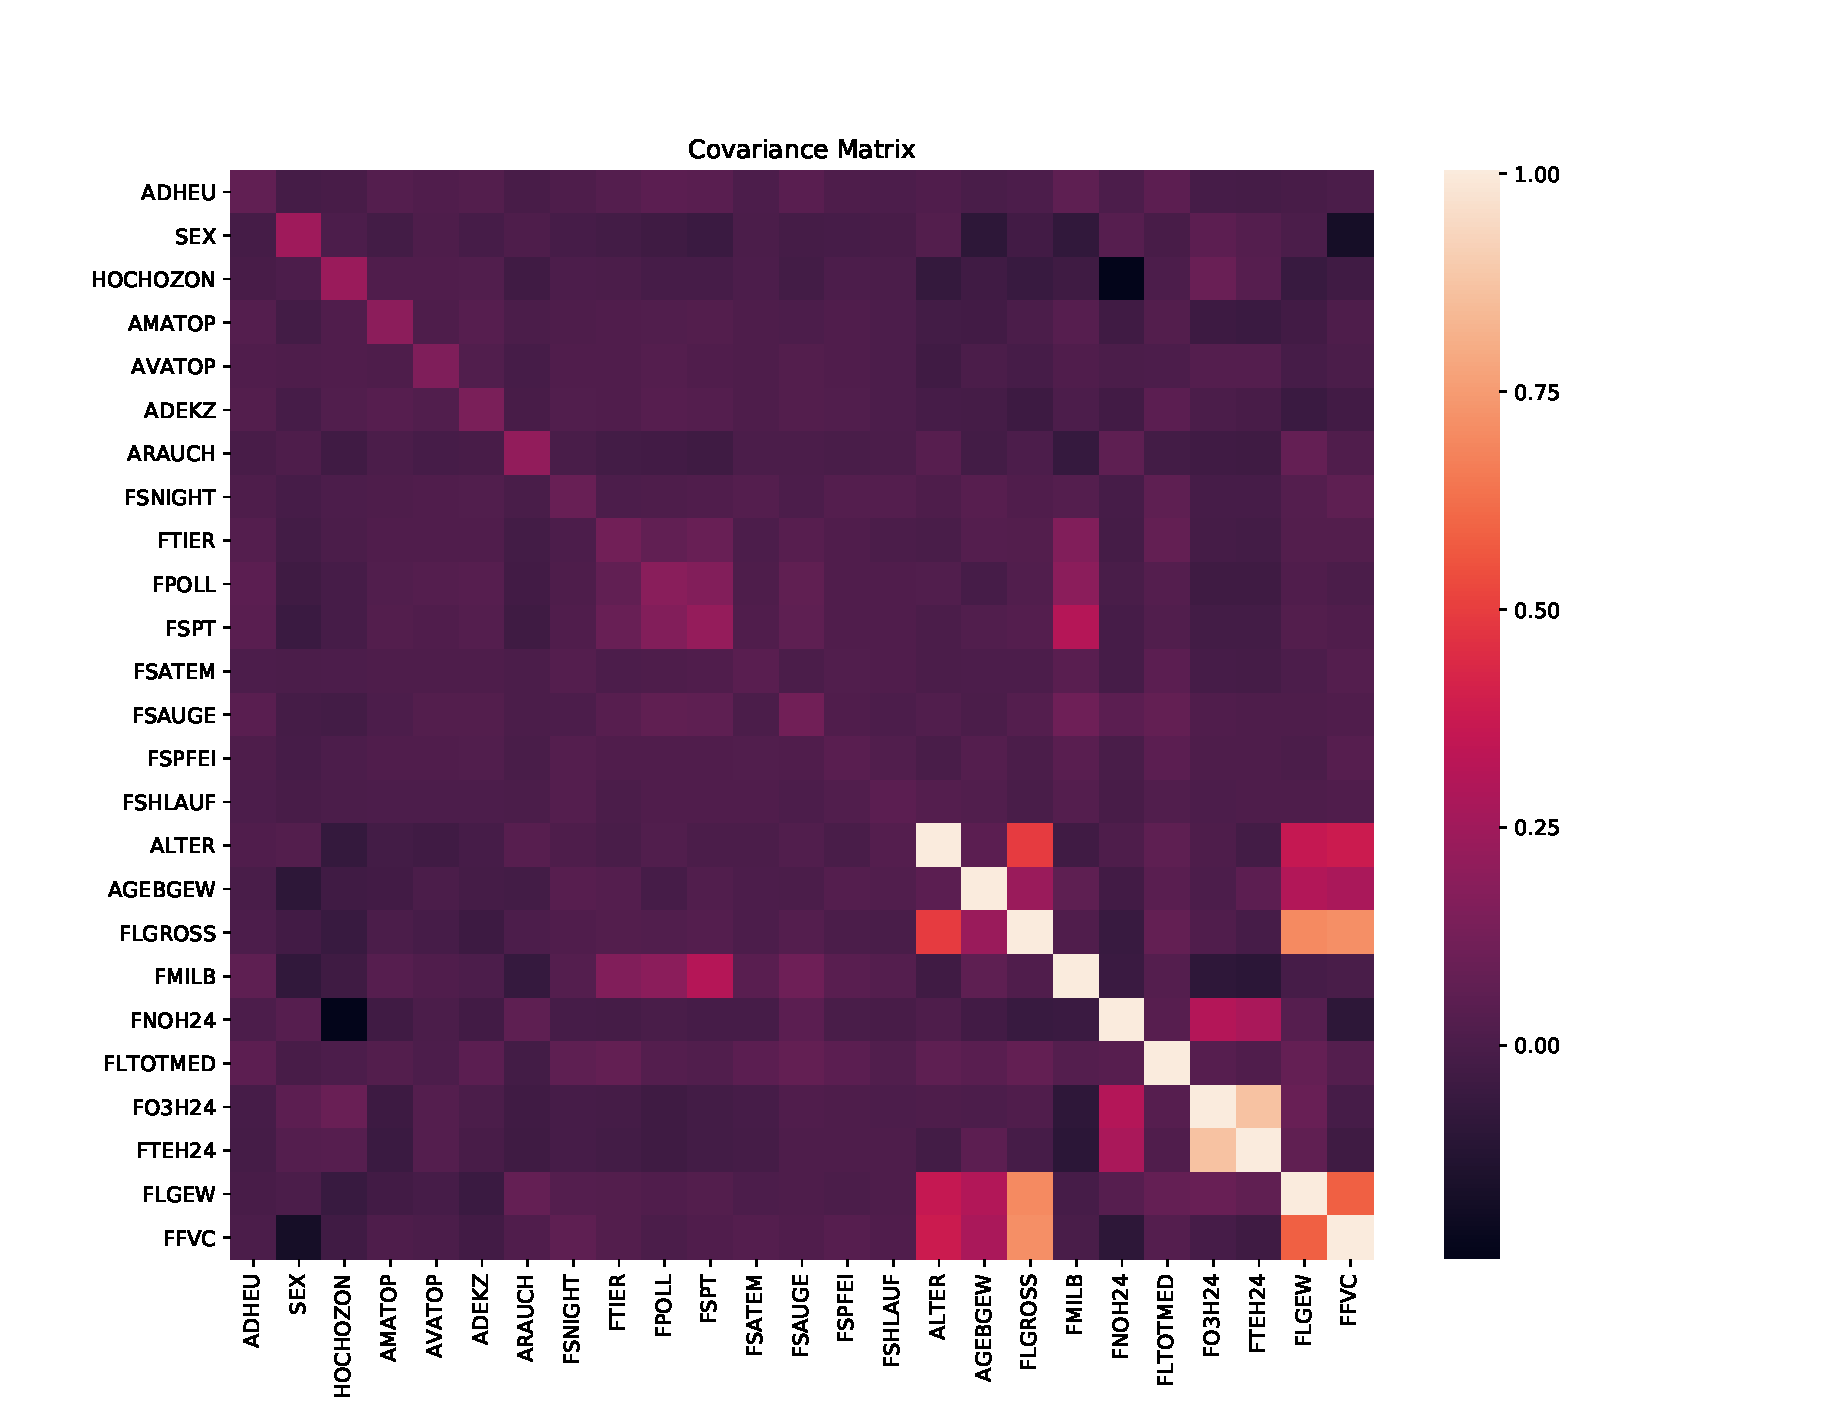
\includegraphics[width=0.8\textwidth]{figures/covheatmap.pdf}
%	\caption{The correlation matrix of the data}
%	\label{fig:corrE1}
%\end{figure}
%Figure \ref{fig:corr_FFVC_E1} illustrates the correlation vector of the FFVC feature:
%\begin{figure}[H]
%	\centering
%	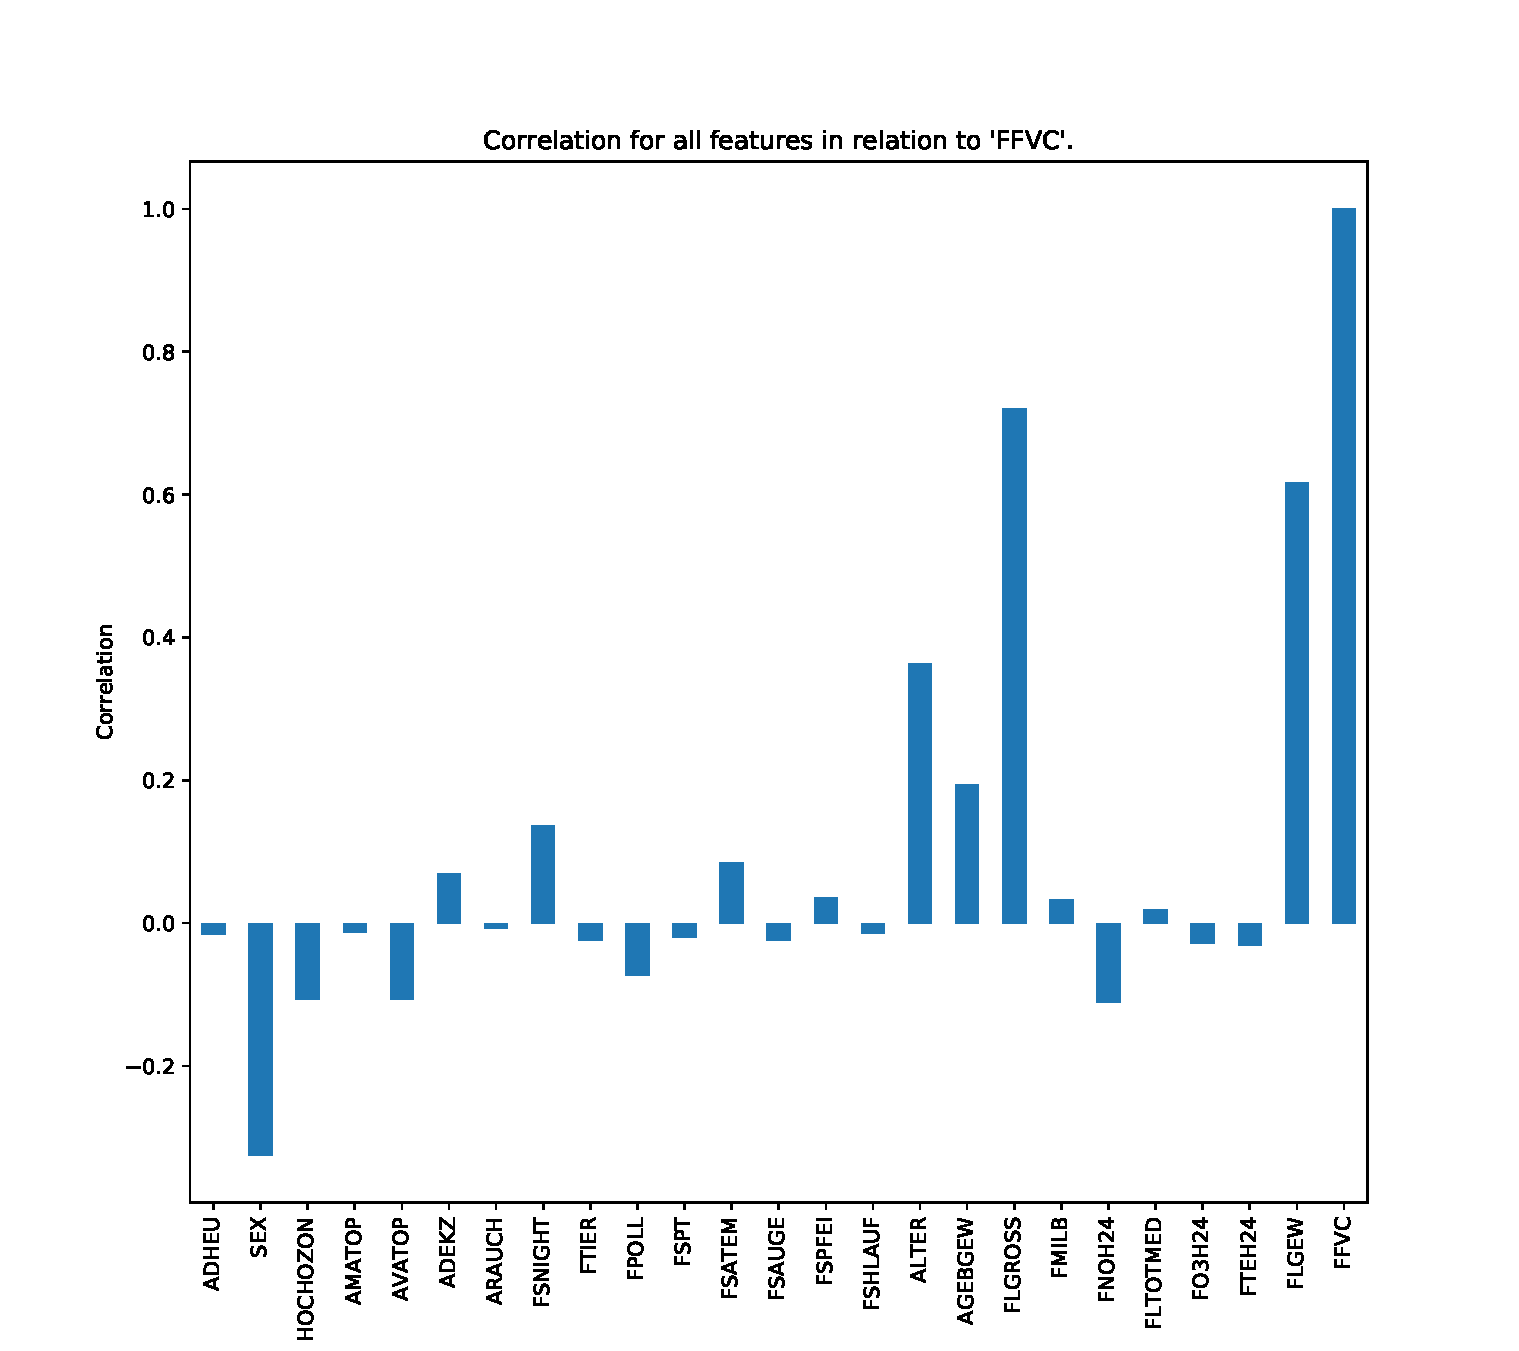
\includegraphics[width=0.8\textwidth]{figures/corr_FFVC_specific.pdf}
%	\caption{The specific correlation of the FFVC features.}
%	\label{fig:corr_FFVC_E1}
%\end{figure}
The covariate which has the strongest association with the forced vital capacity (FFVC) is the FLGROSS feature. Following is a report on the coefficient estimates, their standard error and the associated p-values:
\begin{figure}[H]
	\centering
	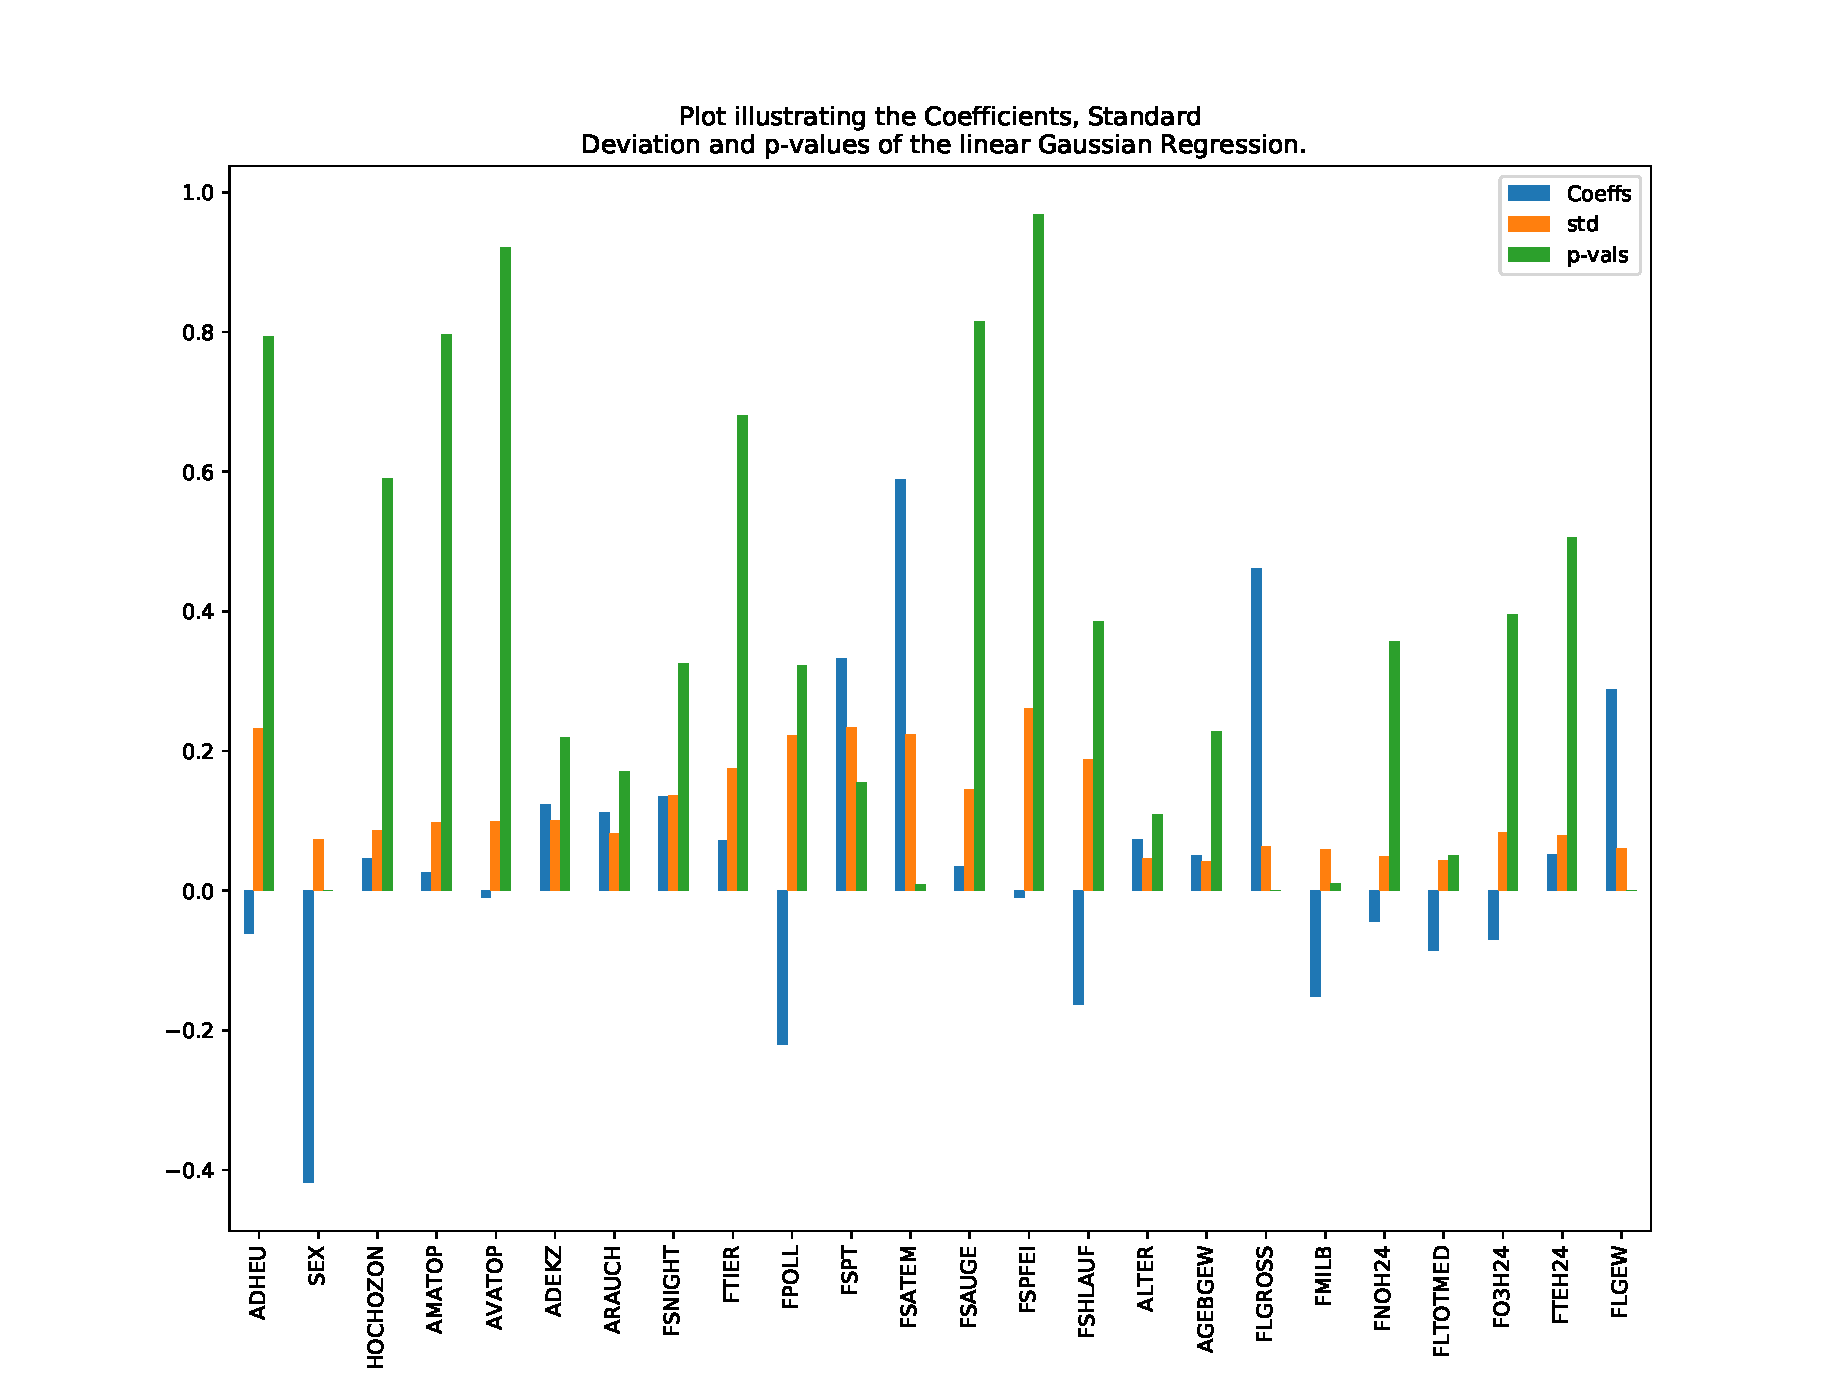
\includegraphics[width=0.8\textwidth]{figures/coefs_std_pvals.pdf}
	\caption{Figure illustrating the coefficients, standard deviations and p-values of all the features.}
	\label{fig:coefs_std_pval}
\end{figure}
It is clear that several of the p-values are quite large in relation to the typical p-value standard of $\sim 0.05$. It is also quite interesting to see in one figure the relation between the coefficient size and the p-value. It is clear to see for the 'SEX' and 'FSATEM' columns that the bigger the regression coefficient, the smaller the p-value of the feature. This can also be seen in the 'FLGROSS' column, which we remember from the covariance matrix as having the strongest association with the 'FFVC'. The opposite is also noticeable; the largest p-values, namely the 'FSPEI' and 'AVATOP' columns have coefficient values close to zero.\\\\ 
Some features do not exhibit this trend, such as the 'FSPT' and 'FPOLL' features exist somewhere in between, where they are not quite relevant to the prediction, but not quite irrelevant either.

\subsection*{3.}
The backwards and forwards selection algorithms performed using two different stopping criterion: One was 0.05 and the other was 0.1. Following are four figures of all these cases, where the coefficients, standard deviations, and all the p-values are listed in the same way as before.
\begin{figure}[H] 
	\label{ fig7} 
	\begin{minipage}[H]{0.5\linewidth}
		\centering
		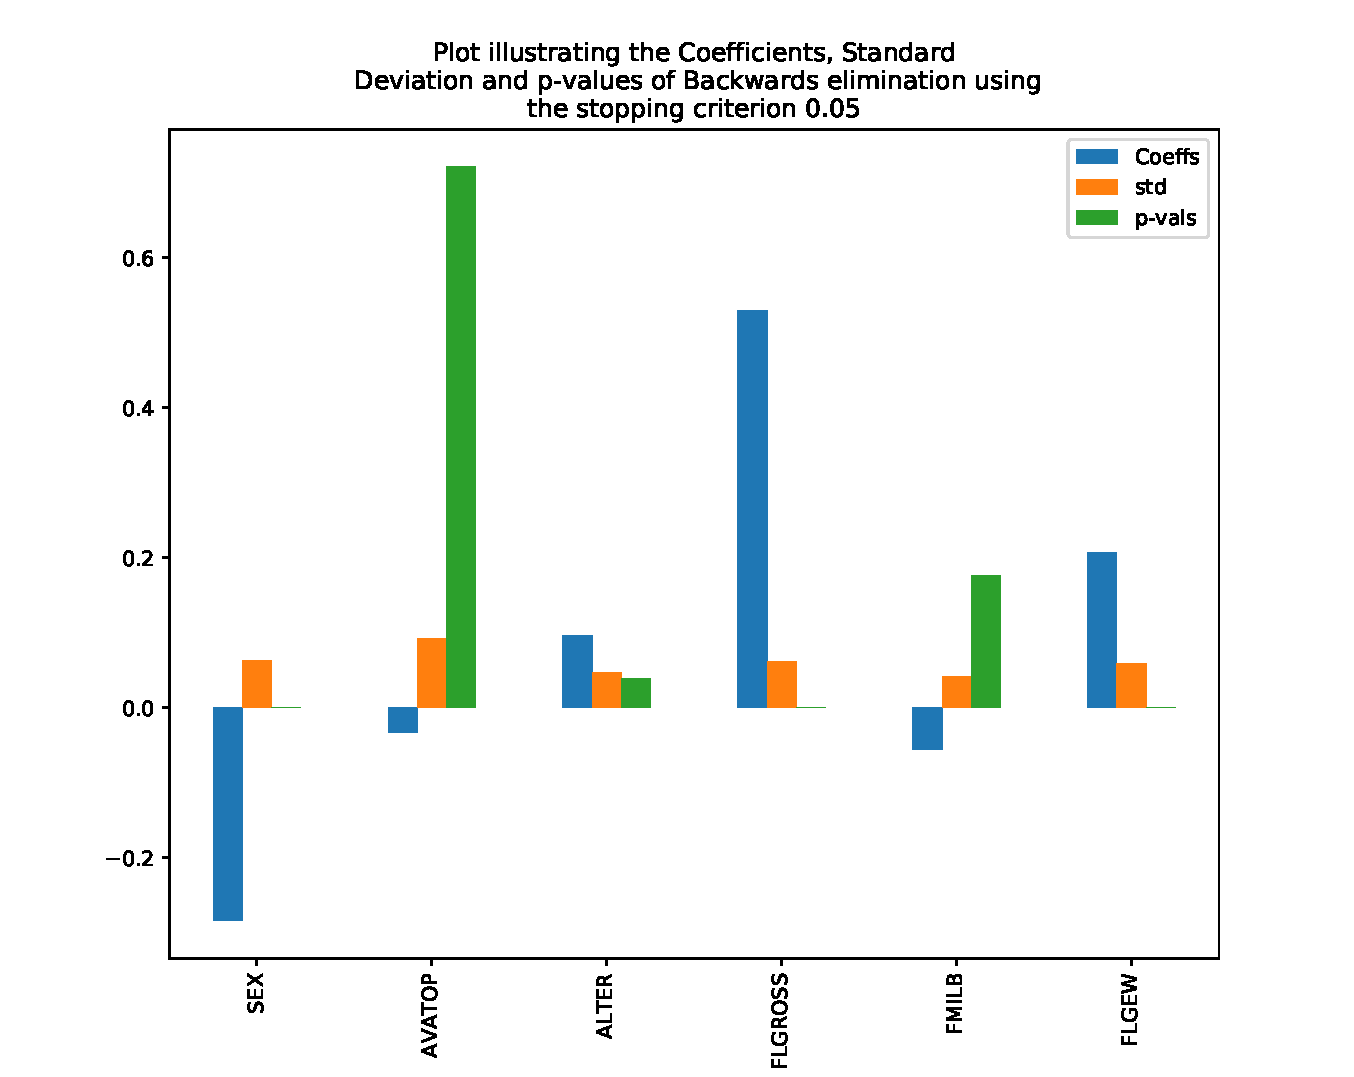
\includegraphics[width=1.11\linewidth]{figures/BS_005.pdf}
		\vspace{4ex}
	\end{minipage}%%
	\begin{minipage}[H]{0.5\linewidth}
		\centering
		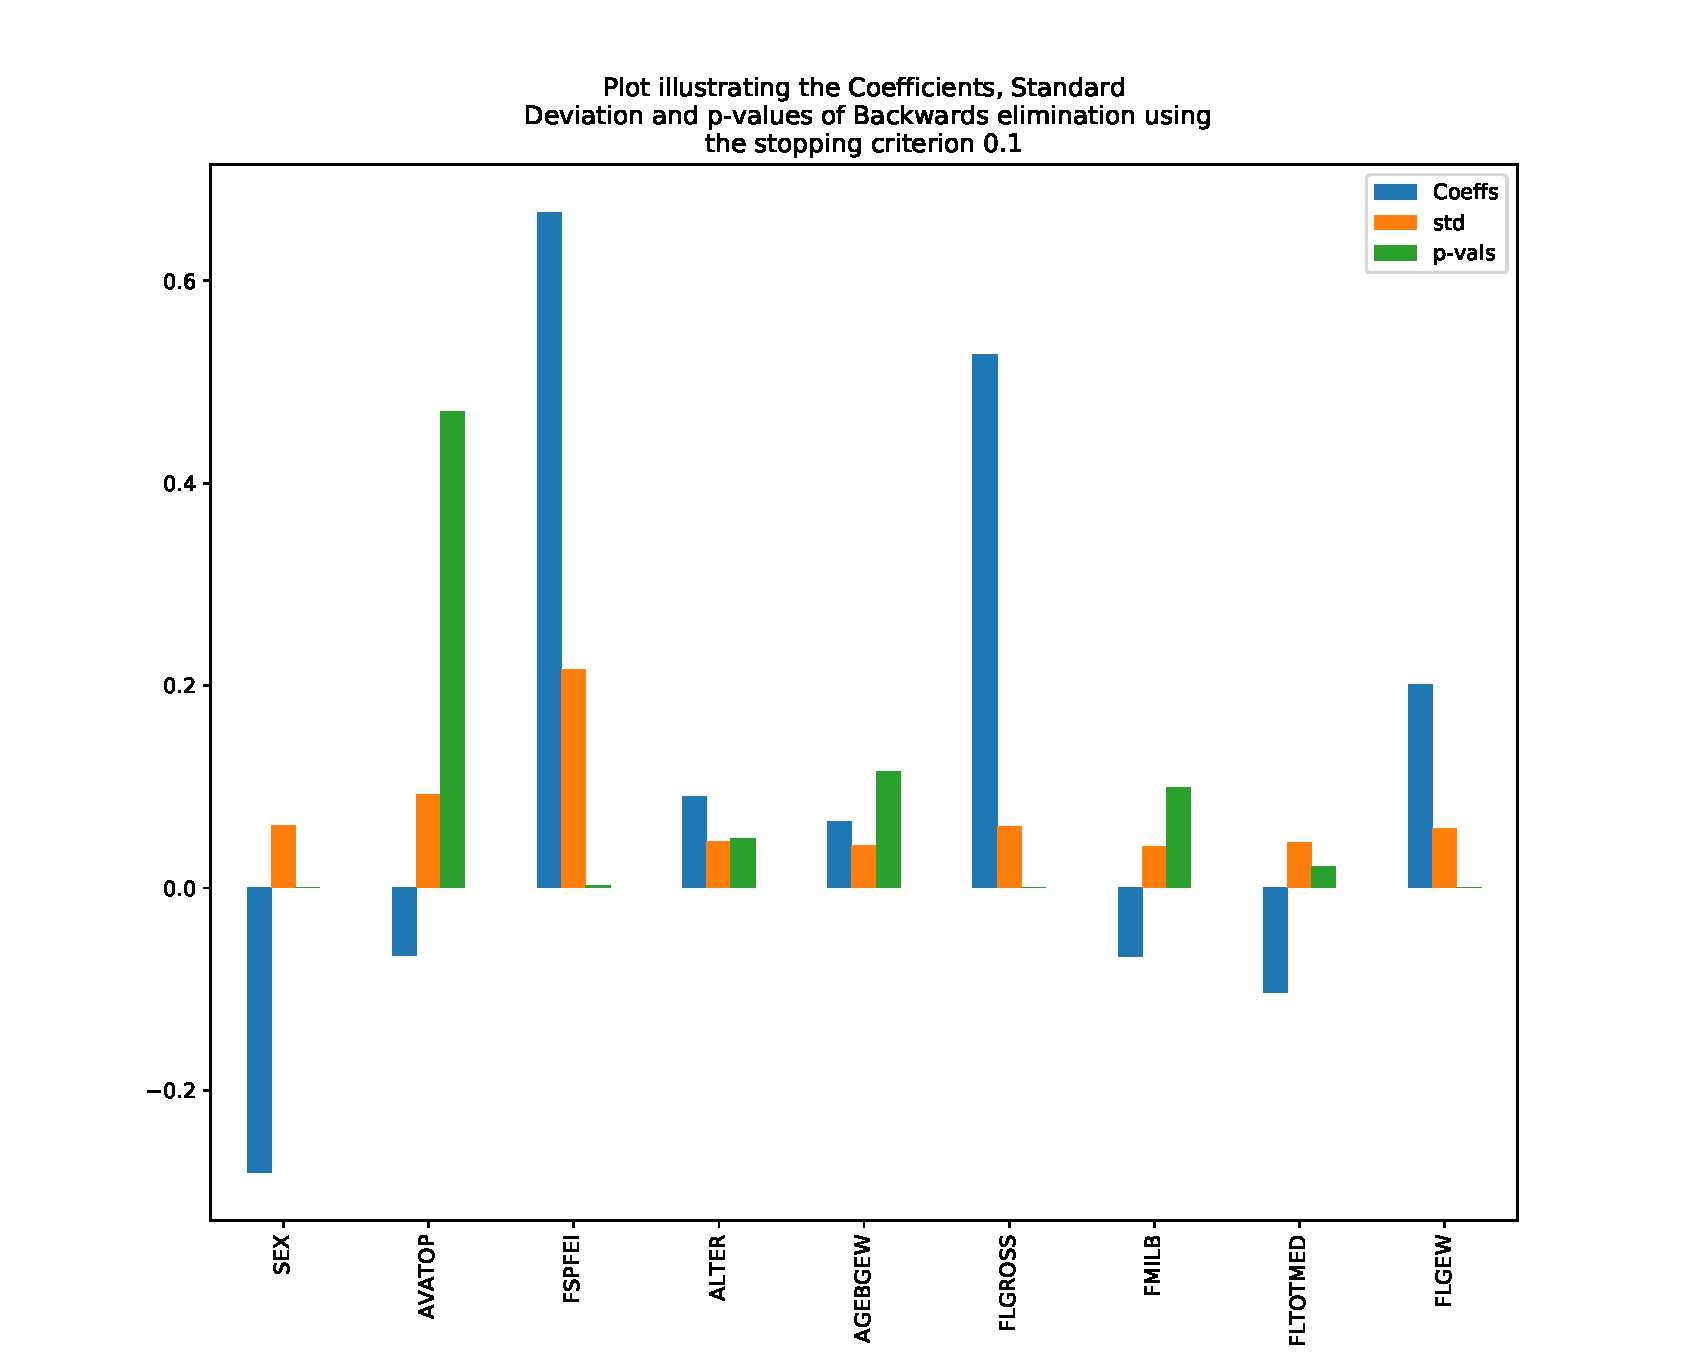
\includegraphics[width=1.11\linewidth]{figures/BS_01.pdf}
		\vspace{4ex}
	\end{minipage} 
	\begin{minipage}[H]{0.5\linewidth}
		\centering
		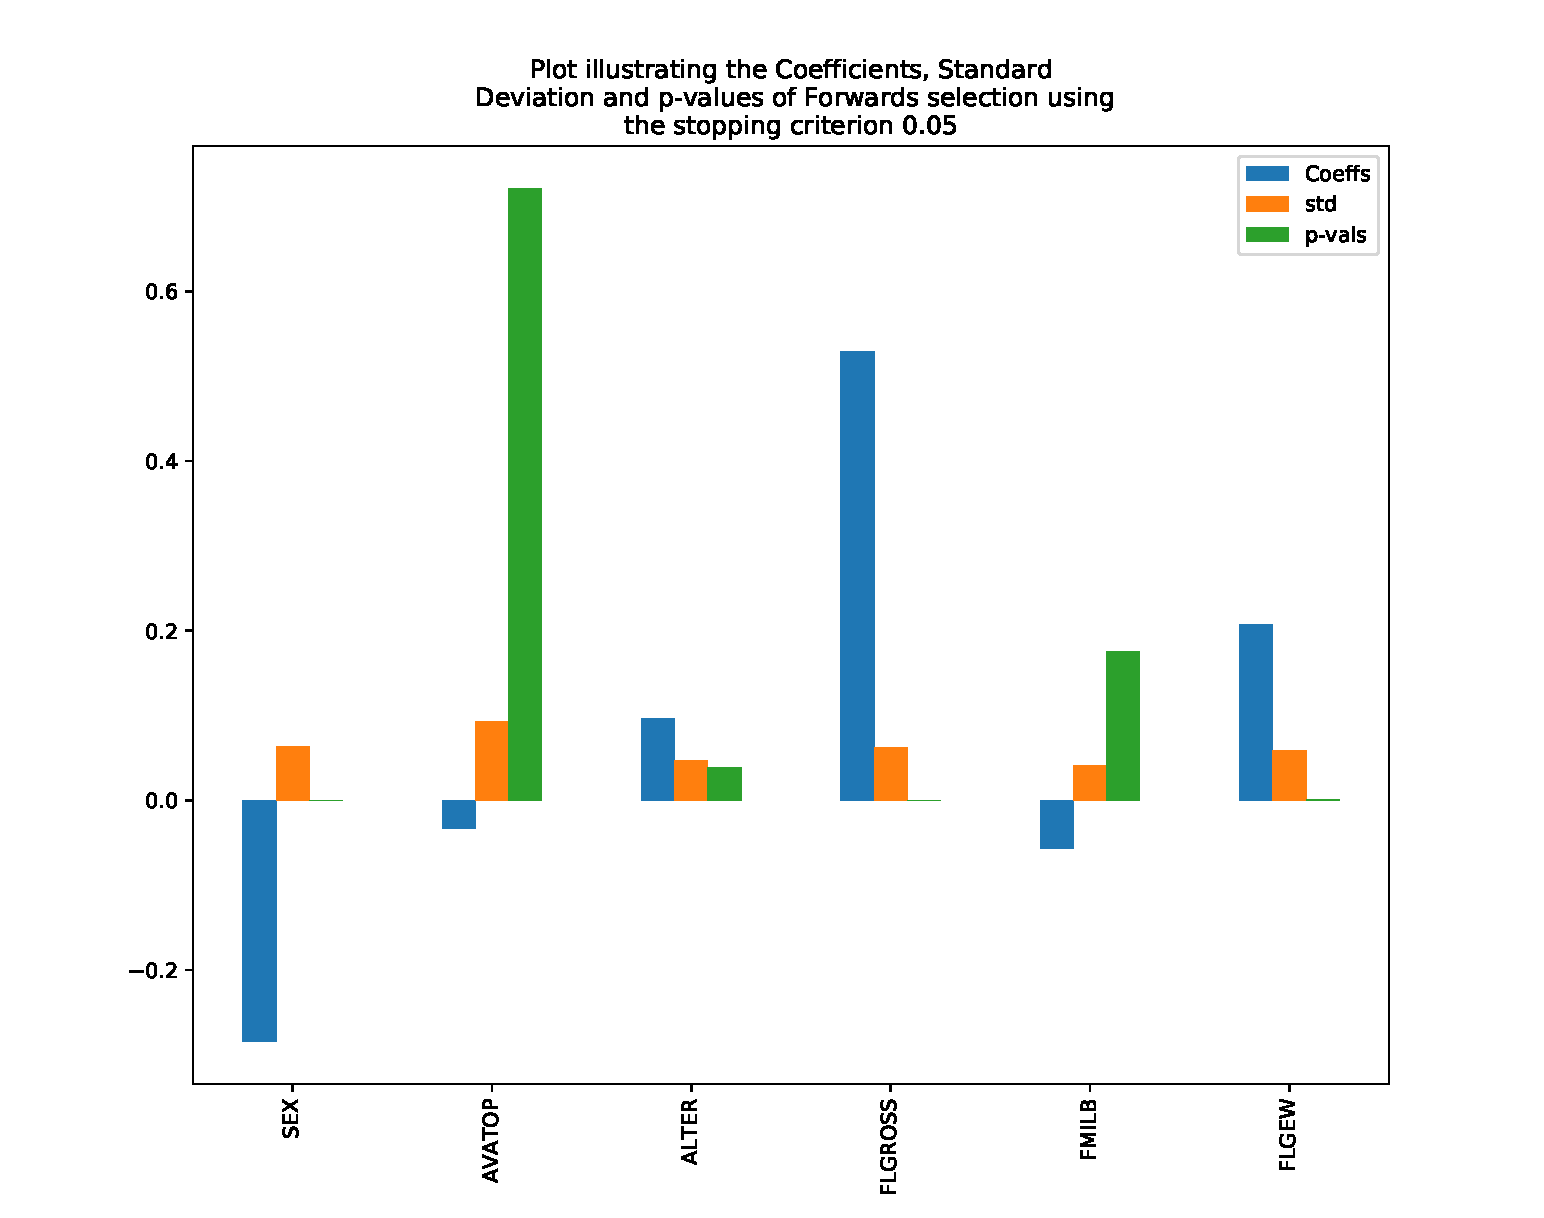
\includegraphics[width=1.11\linewidth]{figures/FS_005.pdf}
		\vspace{4ex}
	\end{minipage}%% 
	\begin{minipage}[H]{0.5\linewidth}
		\centering
		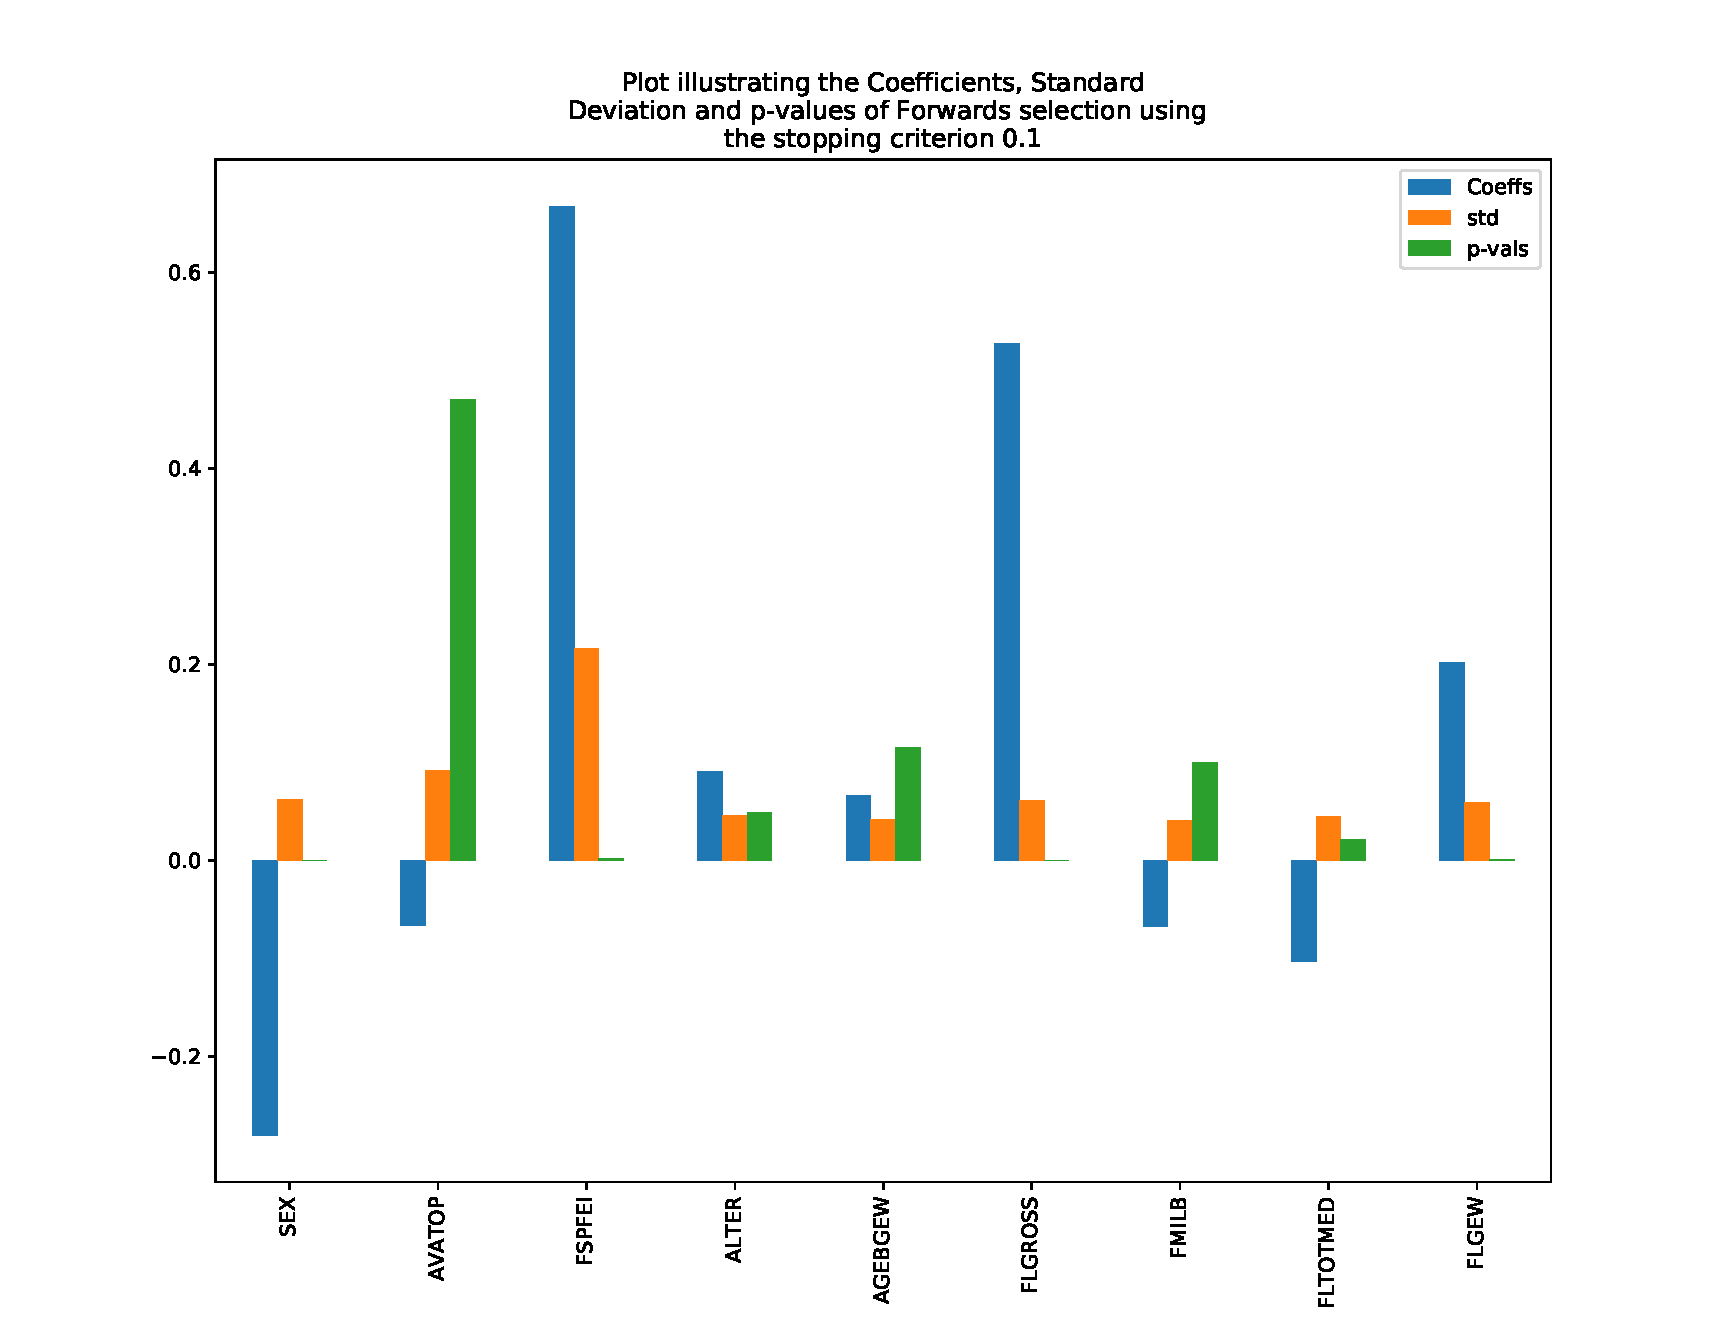
\includegraphics[width=1.11\linewidth]{figures/FS_01.pdf}
		\vspace{4ex}
	\end{minipage} 
\end{figure}
These are all quite similar predictions, as the backwards elimination and forwards selection essentially perform the same operation. They simply set a limit to the p-values, and filter out accordingly.\\\\
These methods are implemented in order to build a high quality regression model with little to no unnecessary features. This is done in a way that hopefully does not compromise the predictive abilities of the model, though some line must be drawn on this subject. Even features such as the 'FTIER' feature (see figure \ref{fig:coefs_std_pval}) helped in predicting the model somewhat. Although it was a feature that seemed to be quite linearly dependent, it still had some use. Removing this feature is not severely jeopardizing to the model's prediction, though some accuracy is lost. I therefore hypothesize that the mean-squared error will overall increase after the backwards elimination and forwards selection techniques.\\\\
Note, that when reproducing the following figures, there is a large amount of stochasticity in the data shuffling method. This means that the outcomes sometimes differ quite largely from one and other, so the figures illustrated in this report are simply one of many different cases.

\subsection*{4.}
Use both a bootstrap and k-fold CV method to find the best (in terms of deviance minimization) complexity parameter of a lasso regression.
Following is the bootstrap method results. The data was split up into 50/50, and the training data was further split up into $25\%$ testing data for the bootstrap samples. The $R^2$ scores were calculated using the average of a lot of bootstrap samples, for multiple hyperparameter $\alpha$ values. Figure \ref{fig:bootstrapE1} illustrates the results of this analysis:
\begin{figure}[H]
	\centering
	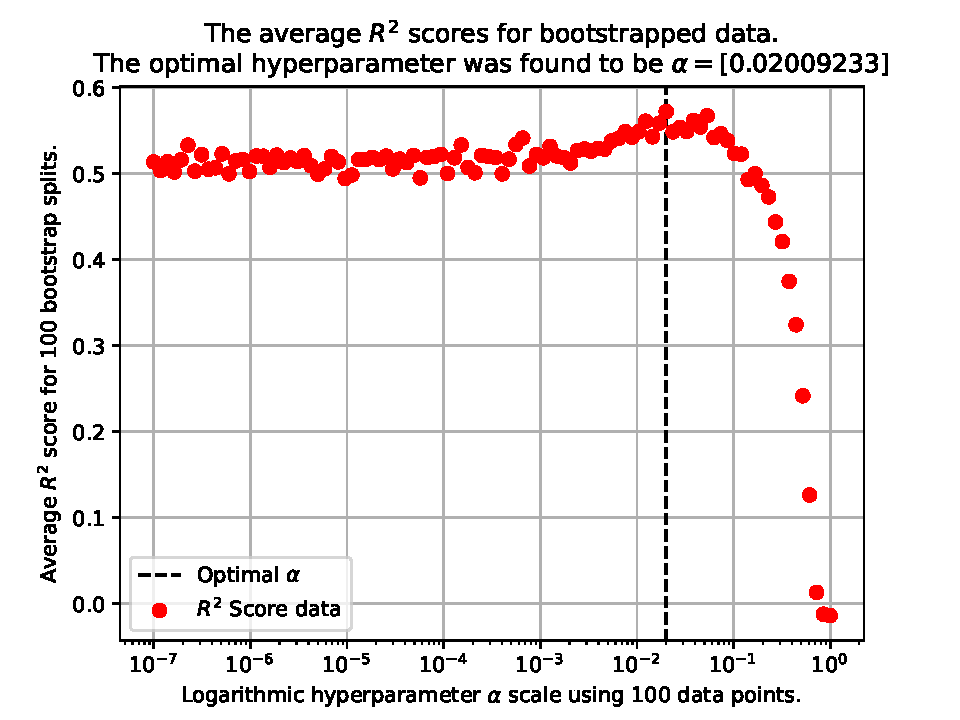
\includegraphics[width=0.8\textwidth]{figures/Bootstrap_E1.pdf}
	\caption{Figure illustrating the averages of the $R^2$ scores of multiple bootstrap samples. The optimal $\alpha$ parameter is found to be $\alpha=0.02$.}
	\label{fig:bootstrapE1}
\end{figure}

Doing the same for 5-fold CV, the two optimal $R^2$ scores are generated:

\begin{table}[H]
	\centering
	\caption{Maximum $R^2$ scores and minimum MSE scores of the two methods.}
	\begin{tabular}[t]{l@{\hskip 0.5in}c@{\hskip 0.5in}c}
		\toprule
		Scheme & Bootstrap & 5-fold CV \\
		\midrule
		 & & \\
		$R^2$ & 0.64222 & 0.56684 \\
		\bottomrule
	\end{tabular}
	\label{tab:E1P4}
\end{table}

\subsection*{5.}
Following are the results from the GAM simulations:

Only linear terms:
\begin{figure}[H]
	\centering
	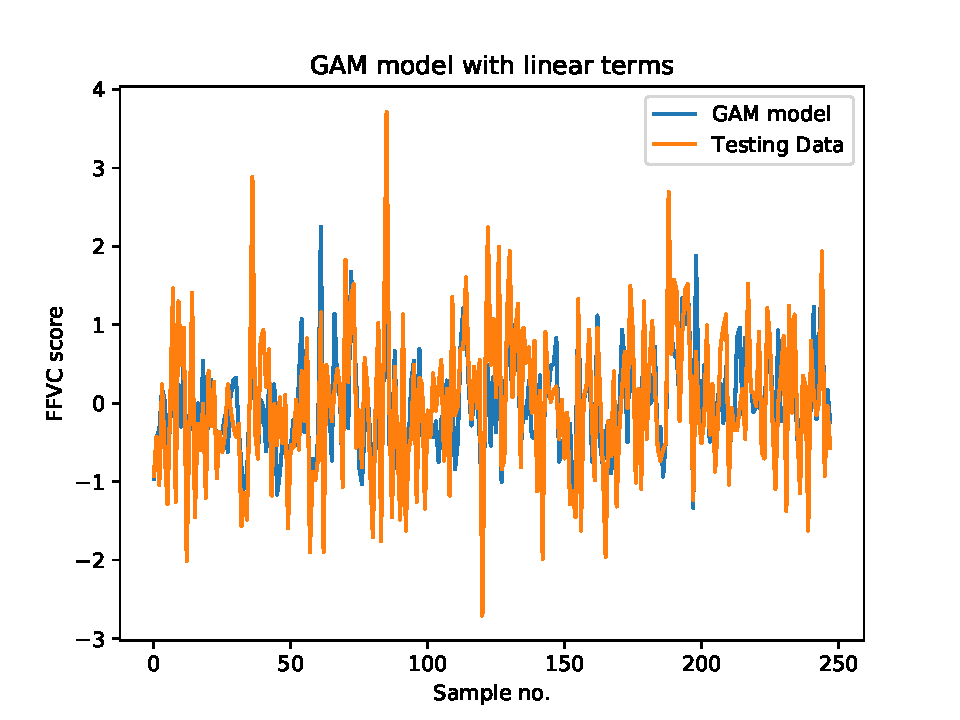
\includegraphics[width=0.8\textwidth]{figures/GAM1_E1.pdf}
	\caption{Figure illustrating the true FFVC scores vs the predicted scores using a GAM with only linear terms.}
	\label{fig:GAM1E1}
\end{figure}
Spline terms allowed:
\begin{figure}[H]
	\centering
	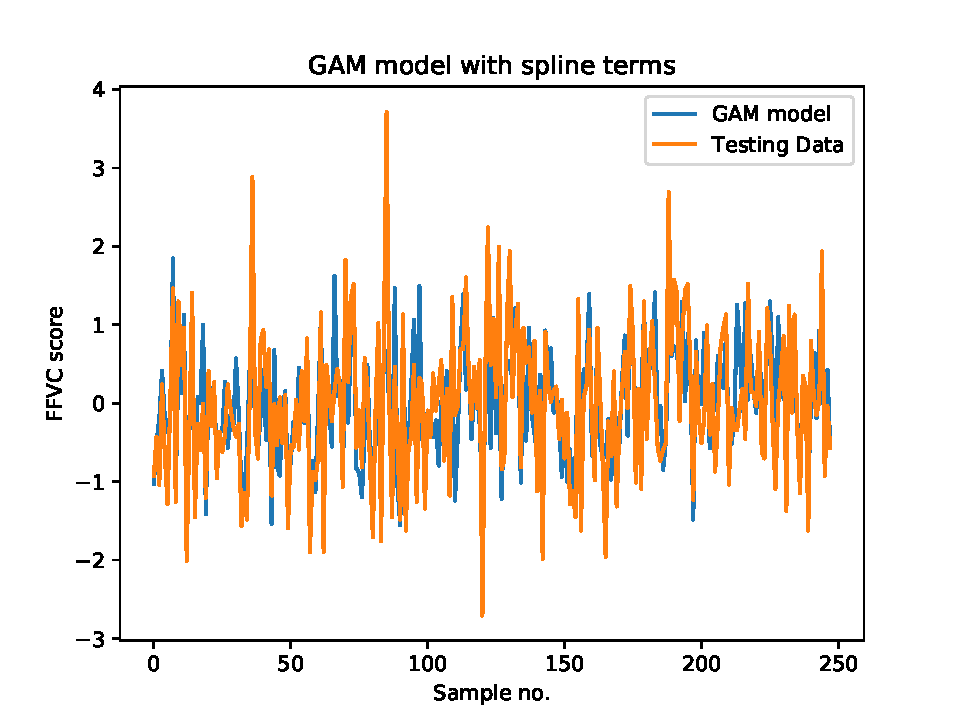
\includegraphics[width=0.8\textwidth]{figures/GAM2_E1.pdf}
	\caption{Figure illustrating the true FFVC scores vs the predicted scores using a GAM with splined, linear and polynomial terms.}
	\label{fig:GAM2E1}
\end{figure}
The 'only linear' GAM produced an MSE of 0.43756327\\

The 'splines and polynomial degrees allowed' GAM produced an MSE of 0.45348646.\\

These results are very chance-dependent, but in general the results are not too far off.

\subsection*{6.}
All the methods were successfully implemented using sklearns utilities. The results are illustrated in both the code and in the following section:

\subsection*{7.}
Following are the results of the code.


Linear Gauss of Exercise 1:
$$
MSE = 1.392
$$
Backwards- and Forwards models of Exercise 2:
MSE of Backwards Elimination 1 and 2:
$$
MSE1 = 1.377 
$$
and 
$$
MSE2 = 1.377
$$
MSE of Forwards Selection 1 and 2:
$$
MSE1 = 1.377
$$ 
and 
$$
MSE2 = 1.377
$$

Lasso results of Exercise 4:
Bootstrap achieved R² = 0.617
5-fold CV achieved R² = 0.553
GAM analysis from Exercise 5:
Linear only model MSE = 0.343
Polynomial allowed model MSE = 0.441
3 boosting models of Exercise 6:
i)   : MSE = 1.446
ii)  : MSE = 0.000
iii) : MSE = 1.378


\section*{Exercise 2}
\subsection*{1.}
Figure \ref{fig:cumgains_kNN} illustrates the cumulative gains curve generated by the k-Nearest Neighbor method using $k=10$ and $33\%$ testing data.
\begin{figure}[H]
	\centering
	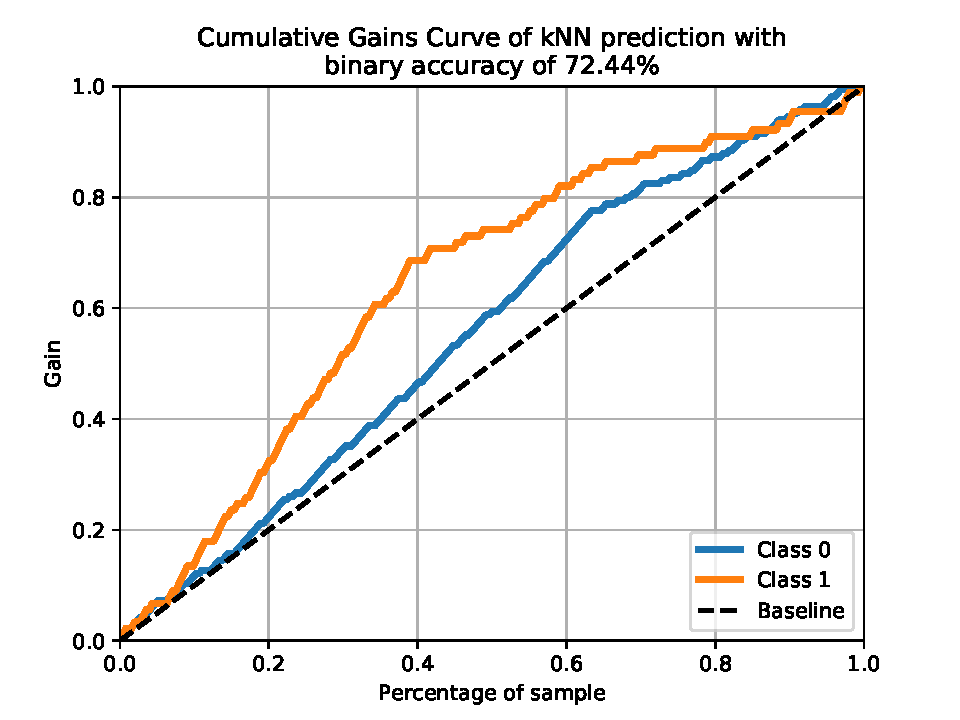
\includegraphics[width=0.8\textwidth]{figures/kNN_E2P1.pdf}
	\caption{Figure illustrating the averages of the $R^2$ scores of multiple bootstrap samples. The optimal $\alpha$ parameter is found to be $\alpha=0.02$.}
	\label{fig:cumgains_kNN}
\end{figure}
Figure \ref{fig:kNN_k} illustrates an analysis of which k value produces the optimal score:
\begin{figure}[H]
	\centering
	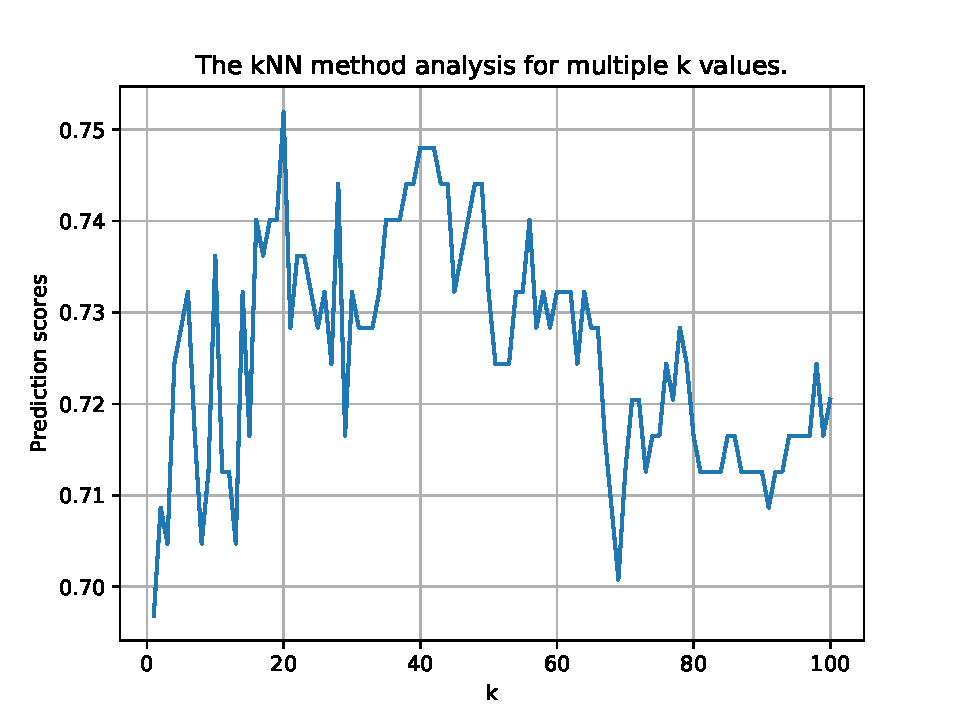
\includegraphics[width=0.8\textwidth]{figures/E1P2_kNN.pdf}
	\caption{Figure illustrating the averages of the $R^2$ scores of multiple $k$ values.}
	\label{fig:kNN_k}
\end{figure}

\subsection*{2.}
Figure \ref{fig:GAMRES} illustrates the prediction results for the GAM method using splines only. 
\begin{figure}[H]
	\centering
	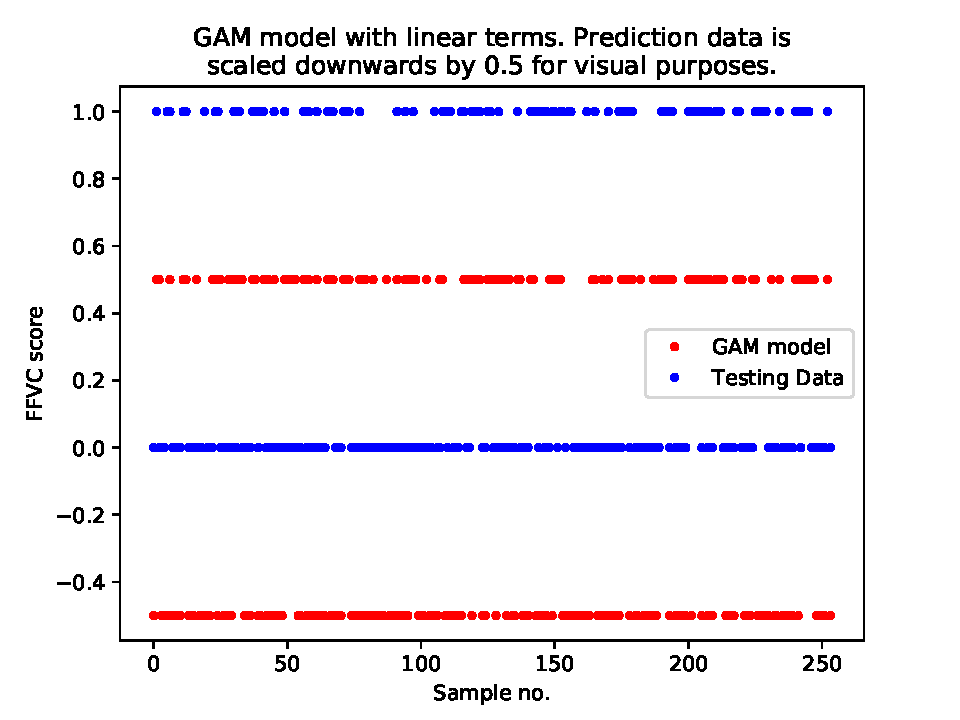
\includegraphics[width=0.8\textwidth]{figures/GAM_RESULTS.pdf}
	\caption{GAM results for exercise 2.}
	\label{fig:GAMRES}
\end{figure}

\subsection*{3.}
This was implemented into the python program using sklearn's functionalities. Bagging with both voting and averaging was unfortunately not accomplished, however.

\subsection*{4.}
Table \ref{tab:ALMOST} illustrates the results of all these methods.
\begin{table}[H]
	\centering
	\caption{Scores for all the methods from exercise 3.}
	\begin{tabular}[t]{l@{\hskip 0.5in}c}
		\toprule
		Scheme & Score \\
		\midrule
		Decision Tree score:&	 0.6654\\
		Bagging score:  	 &0.7244\\
		Random Forest score:&	 0.7244\\
		Neural Network score:&	 0.7047\\
		ADA Boost score:	 &0.7047\\
		\bottomrule
	\end{tabular}
	\label{tab:ALMOST}
\end{table}


If I were to choose between these models, I would choose the bagging or the random forest method. This choice is due to the score performances. However, all these methods are very reliable, and upon multiple runs of the code, they are all found to have large deviations (oscillations) depending on the randomness seed. This would be interesting to study further.


\subsection*{5.}
Following are the new figures, just with the outliers removed. The figures illustrate the same phenomenon as before:
\begin{figure}[H]
	\centering
	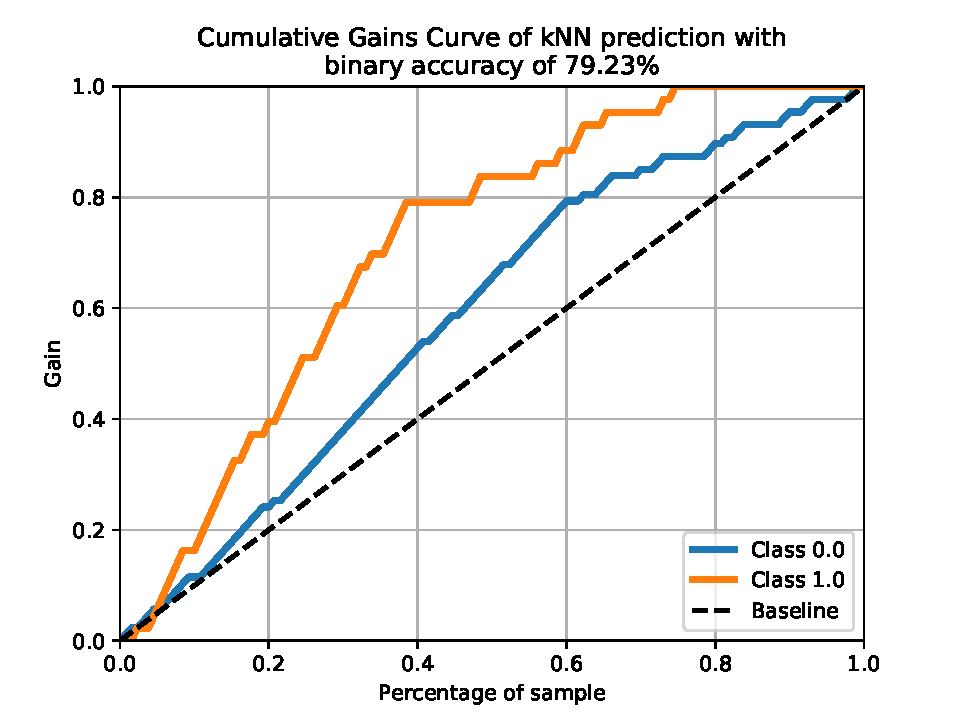
\includegraphics[width=0.8\textwidth]{figures/LASTONE.pdf}
	\label{fig:LASTONE}
\end{figure}
\begin{figure}[H]
	\centering
	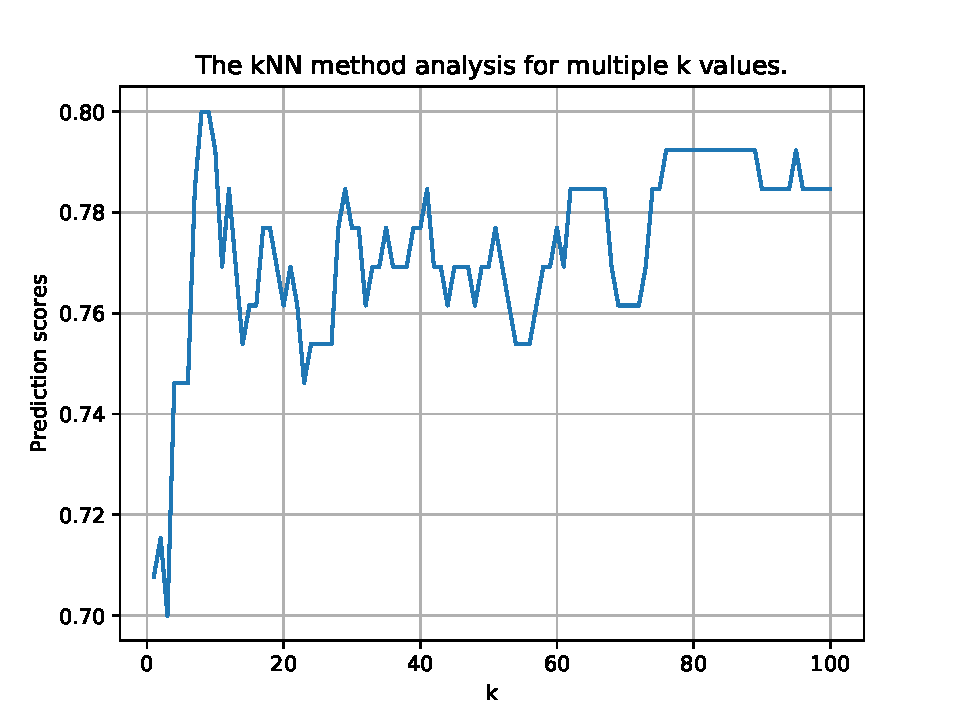
\includegraphics[width=0.8\textwidth]{figures/LASTTWO.pdf}
	\label{fig:LASTTWO}
\end{figure}
\begin{figure}[H]
	\centering
	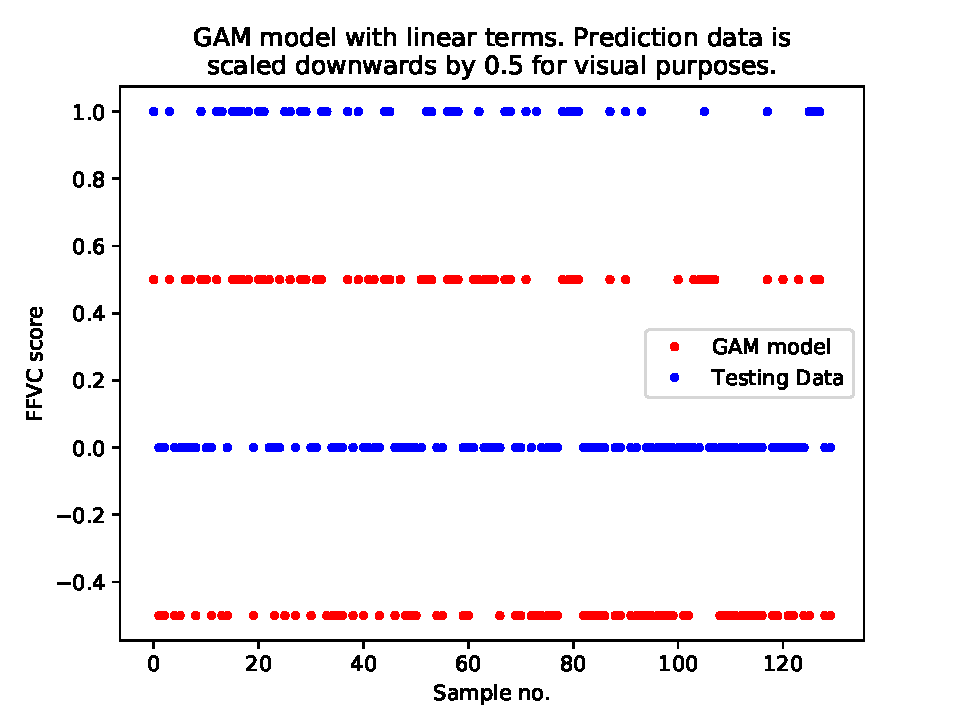
\includegraphics[width=0.8\textwidth]{figures/LASTTHREE.pdf}
	\label{fig:LASTTHREE}
\end{figure}

Following are the results again:

\begin{table}[H]
	\centering
	\caption{Scores for all the methods with outliers removed.}
	\begin{tabular}[t]{l@{\hskip 0.5in}c}
		\toprule
		Scheme & Score \\
		\midrule
		Decision Tree score:&	 0.6692\\
		Bagging score:  	& 0.7385\\
		Random Forest score:&	 0.7923\\
		Neural Network score:&	 0.7462\\
		ADA Boost score:	 &0.7385\\
		\bottomrule
	\end{tabular}
	\label{tab:LASTONE}
\end{table}




% References
\section*{References}
McLeod, S. A. (2019, May 20). What a p-value Tells You About Statistical significance. Simply Psychology. https://www.simplypsychology.org/p-value.html

\end{document}
